\section{Results I: the counting laws hold, and the verdict reverses}\label{sec:attention}

\subsection{The entry law is exact, and linearity is an artefact of the grid}

Table~\ref{tab:counting} compares \eqref{eq:entrylaw} with the measured number of
attended entries on the grid $n\in\{256,512,1024,2048,4096\}$, with $w=\WinW$,
$g=\AnchorG$, $s=\Sinks$. The two agree at every length: the relative deviation is
\NnzLawMaxErrPct\%, i.e. the identity is exact rather than asymptotic. The
leading-order form \eqref{eq:entryasym} is also tabulated; it is the form a
designer would use, and it overstates the count by $15\%$ at $n=256$ and by
$1.2\%$ at $n=4096$, which is the size of the remainder it discards.

\begin{table}[t]
\centering
\begin{tabular}{rrrrrr}
\toprule
$n$ & measured & Eq.~\eqref{eq:entrylaw} & rel.\ err & asymptotic & density \\
\midrule
256 & 15{,}226 & 15{,}226 & +0.000\% & 17{,}600 & 46.29\% \\
512 & 33{,}370 & 33{,}370 & +0.000\% & 35{,}861 & 25.41\% \\
1{,}024 & 71{,}674 & 71{,}674 & +0.000\% & 74{,}432 & 13.66\% \\
2{,}048 & 156{,}506 & 156{,}506 & +0.000\% & 159{,}765 & 7.46\% \\
4{,}096 & 358{,}906 & 358{,}906 & +0.000\% & 363{,}200 & 4.28\% \\
\bottomrule
\end{tabular}

\caption{Entry law. Measured number of attended entries against the identity
\eqref{eq:entrylaw} and against its asymptotic form
$n(w+s)+(n-w)^2/(2g)$, with $w=\WinW$, $g=\AnchorG$, $s=\Sinks$. The identity is
exact on the whole grid, so the residual column is zero to three decimals; the
asymptotic form carries the stated remainder. The last column is the entry count as
a fraction of the causal matrix. Data:
\texttt{s1\_pswa/complexity\_curve.json}.}
\label{tab:counting}
\end{table}

The fitted log-log slope of the measured count is $\NnzSlopeFitted$ over this
grid, comfortably below the dense value of two, and it is tempting to report that
number as evidence of sub-quadratic cost. It is not, and
Figure~\ref{fig:counting} shows why. The local exponent, evaluated between
consecutive lengths, moves from $\NnzLocalExponentMin$ to $\NnzLocalExponentMax$
across the grid, because the window term still dominates below
$n^\ast=\CrossoverLen$ (Equation~\eqref{eq:crossover}); the exponent of the closed
form, extrapolated with no additional measurement, passes $1.8$ by $n=2^{15}$ and
converges to two. A benchmark that stops at $n=4096$ therefore certifies
linearity that \eqref{eq:entryasym} says cannot hold at $n=\LargestN$, and the
device measurements below are taken exactly where the crossover has been crossed.

\begin{figure}[t]
\centering
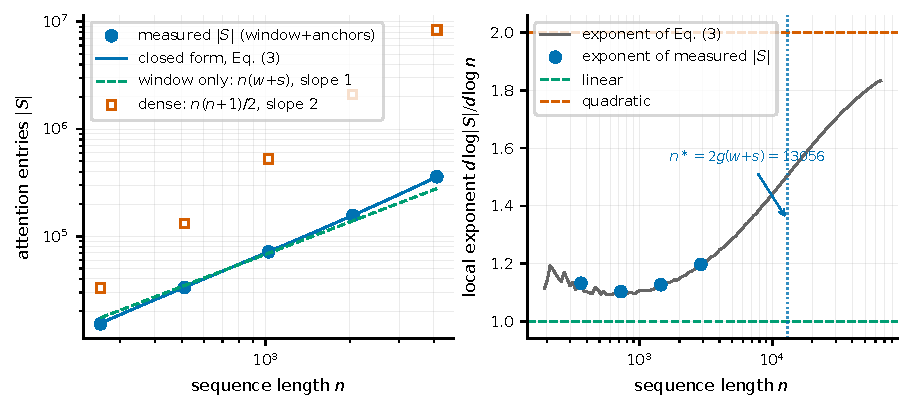
\includegraphics[width=\textwidth]{fig2_counting.pdf}
\caption{Left: attended entries against the closed form \eqref{eq:entrylaw}, the
window-only term $n(w+s)$ (slope one) and the dense count $n(n+1)/2$ (slope two).
Right: local log-log exponent of the entry count. Points are measured; the solid
curve is the exponent of the closed form, plotted beyond the measured grid to show
where it reaches the quadratic regime, and the dotted line marks the crossover
$n^\ast=\CrossoverLen$ of Equation~\eqref{eq:crossover}. The exponents of the
measured points are computed between consecutive lengths, not fitted across the
whole grid. Data: \texttt{s1\_pswa/complexity\_curve.json}.}
\label{fig:counting}
\end{figure}

\subsection{On the device, the anchor variant loses to fused dense attention}\label{sec:device}

Table~\ref{tab:device} and Figure~\ref{fig:device} report peak transient device
memory and median latency for six implementations across five orders of magnitude
of $n$, on the \GpuMemGiB\,GiB device described in Section~\ref{sec:setting}. Four
facts stand out.

\begin{table}[t]
\centering
\resizebox{\textwidth}{!}{\begin{tabular}{rrrrrrrrrrrrr}
\toprule
$n$ & \multicolumn{2}{c}{dense materialised} & \multicolumn{2}{c}{fused SDPA} & \multicolumn{2}{c}{local window} & \multicolumn{2}{c}{local + sinks} & \multicolumn{2}{c}{window + anchors} & \multicolumn{2}{c}{window + anchors, streamed} \\
 & MiB & ms & MiB & ms & MiB & ms & MiB & ms & MiB & ms & MiB & ms \\
\midrule
256 & 0.31 & 0.3 & 0.03 & 0.1 & 0.42 & 1.4 & 0.58 & 1.4 & 0.58 & 1.1 & 0.16 & 2.1 \\
512 & 1.25 & 0.3 & 0.06 & 0.1 & 0.83 & 0.9 & 1.15 & 1.1 & 1.47 & 1.2 & 0.24 & 4.7 \\
1{,}024 & 5.01 & 0.4 & 0.12 & 0.2 & 1.66 & 1.5 & 2.31 & 1.4 & 4.23 & 1.3 & 0.39 & 8.2 \\
2{,}048 & 20.02 & 0.6 & 0.25 & 0.3 & 3.33 & 1.2 & 4.61 & 1.3 & 14.20 & 1.4 & 0.69 & 16.7 \\
4{,}096 & 80.03 & 2.2 & 0.50 & 0.6 & 6.66 & 1.4 & 9.22 & 1.9 & 47.66 & 4.0 & 1.28 & 40.4 \\
8{,}192 & 320.06 & 9.6 & 1.00 & 1.0 & 13.31 & 3.0 & 18.44 & 2.2 & 178.31 & 9.0 & 2.48 & 94.9 \\
16{,}384 & 1{,}280.12 & 26.1 & 2.00 & 2.6 & 26.62 & 3.0 & 36.88 & 3.5 & 682.62 & 28.4 & 4.87 & 271.1 \\
32{,}768 & oom & - & 4.00 & 12.0 & 53.25 & 5.8 & 73.75 & 6.3 & 2{,}677.25 & 108.1 & 10.48 & 870.8 \\
\bottomrule
\end{tabular}
}
\caption{Device measurements on a \GpuName{} (\GpuMemGiB\,GiB, compute capability
\GpuCapability), float16, $d=64$, $B=\GpuBlock$, $w=\GpuW$, $g=\GpuG$, median of
\GpuReps{} repetitions. Memory is the peak transient allocation of the operator
after baseline decontamination (Section~\ref{sec:device_protocol}); \emph{oom}
marks an out-of-memory outcome that is stored as such and not interpolated.
Data: \texttt{s1\_pswa/gpu\_memory\_latency.json}.}
\label{tab:device}
\end{table}

\emph{(i) Memory grows quadratically for the anchor variants and linearly without
them.} The fitted log-log slopes of transient memory against $n$ are
\SlopeDense{} for the naive dense implementation, \SlopeSdpa{} for the fused
kernel, \SlopeSliding{} for a pure window, \SlopeLocal{} for a window plus sinks,
\SlopePswa{} for window plus periodic anchors, and \SlopeStream{} for the
streaming implementation of the same pattern. The two patterns that contain no
periodic anchors are linear; the two that contain them are not. This is
Theorem~\ref{thm:linear} observed directly. What separates the two groups is not
sparsity, since every one of these patterns attends to a vanishing fraction of the
matrix; it is whether the global-key budget is bounded.

\emph{(ii) The absolute numbers decide.} At $n=\LargestN$ the anchor variant
needs \VramPswaBig\,MiB against \VramSdpaBig\,MiB for the fused dense kernel,
i.e. $\VramTimesSdpa\times$ as much, and it is \LatencySlowdownVsSdpa$\times$
slower (\LatPswaBig\,ms against \LatSdpaBig\,ms). The naive dense path runs out of
memory at that length while the sparse path still runs. That is the one comparison
in which the sparse design wins, and it wins against the baseline a real system
would not use. Against the window-plus-sinks pattern, which is the same
family with the anchors deleted, the anchor variant costs
$\MemLocalRatio\times$ the memory and $\LatLocalRatio\times$ the latency
(\VramLocalBig\,MiB, \LatLocalBig\,ms).

\emph{(iii) Dropping the anchors improves both axes.} A pure sliding window with $w=\GpuW$ uses \VramSlidingBig\,MiB and
\LatSlidingBig\,ms at $n=\LargestN$, which is \LatSlidingRatio$\times$
\emph{faster} than the fused dense kernel and two orders of magnitude below the
anchor variant in memory. The quality cost of dropping the anchors is real and is
quantified in Section~\ref{sec:mass}; what the measurement establishes is that the
anchor machinery, as realised in an otherwise identical kernel, buys nothing on the
device and costs everything.

\emph{(iv) The streaming variant trades one pathology for another.} Processing one
query block at a time gives the asymptotically minimal live set, slope
\SlopeStream{} and \VramStreamBig\,MiB at $n=\LargestN$, and pays for it with
launch overhead: \LatStreamBig\,ms, i.e. \LatStreamRatio$\times$ the fused kernel.
The pair of sparse measurements is what makes the comparison honest: a claim of
``linear memory'' and a claim of ``practical speed'' can each be supported, but
not by the same implementation.

\begin{figure}[t]
\centering
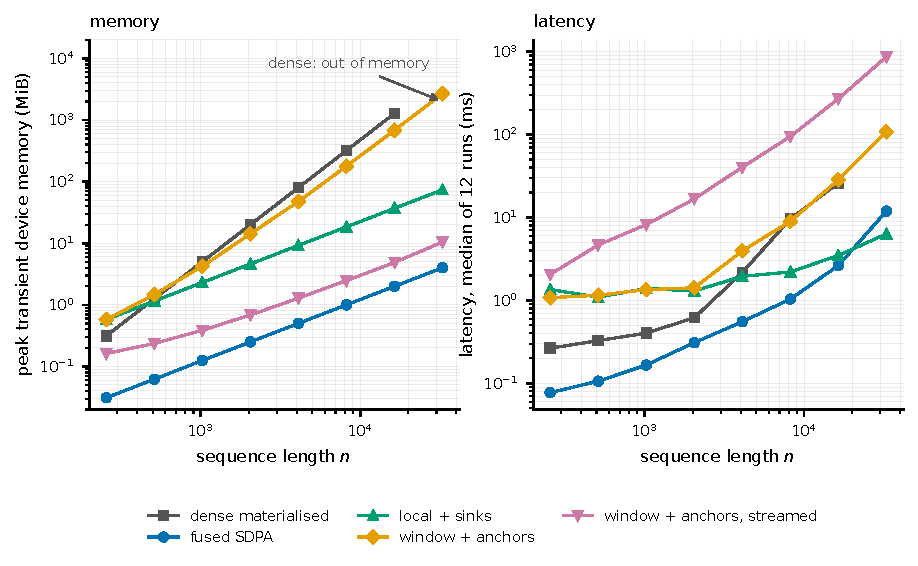
\includegraphics[width=\textwidth]{fig3_device.pdf}
\caption{Peak transient device memory (left) and median latency (right) against
sequence length, log--log, on one \GpuName{}. Slopes: dense materialised
\SlopeDense{}, fused SDPA \SlopeSdpa{}, local window \SlopeSliding{}, local plus
sinks \SlopeLocal{}, window plus anchors \SlopePswa{}, window plus anchors
streamed \SlopeStream{}. The anchor-based variants are the only ones that leave
the linear regime, and they are the only ones that lose to the fused dense kernel.
Data: \texttt{s1\_pswa/gpu\_memory\_latency.json}.}
\label{fig:device}
\end{figure}

\subsection{The kernel executes far more than the mask advertises}\label{sec:granularity}

Table~\ref{tab:block} evaluates \eqref{eq:blocklaw} at $n=\AlignN$,
$B=\AlignBlock$, $w=\AlignW$ for six anchor periods, and
Table~\ref{tab:granularity} varies the block size at a fixed period. The
decomposition is exact: the sum of the anchor term $\min(1,B/g)$ and the measured
window term reproduces the measured block density to three decimals in all six
settings, including the one where $g$ is not a multiple of $B$ and the three where
$g<B$.

\begin{table}[t]
\centering
\begin{tabular}{rrrrrr}
\toprule
$g$ & aligned & $\min(1,B/g)$ & window term & sum & measured \\
\midrule
32 & no & 1.000 & 0.000 & 1.000 & 1.000 \\
96 & no & 0.667 & 0.030 & 0.697 & 0.697 \\
128 & yes & 0.500 & 0.038 & 0.538 & 0.538 \\
192 & yes & 0.333 & 0.051 & 0.384 & 0.384 \\
256 & yes & 0.250 & 0.057 & 0.307 & 0.307 \\
512 & yes & 0.125 & 0.067 & 0.192 & 0.192 \\
\bottomrule
\end{tabular}

\caption{Granularity law \eqref{eq:blocklaw} at $n=\AlignN$, $B=\AlignBlock$,
$w=\AlignW$. The anchor term is $\min(1,B/g)$; the window term is measured; their
sum reproduces the measured block density exactly. Alignment between $g$ and $B$
does not enter the count; the ratio of executed to element density ranges from
\BlockInflationMin{} to \BlockInflationMax{} across the six periods. Data:
\texttt{s1\_pswa/block\_alignment.json}.}
\label{tab:block}
\end{table}

\begin{table}[t]
\centering
\begin{tabular}{rrrrrr}
\toprule
$B$ & aligned & block pairs & causal blocks & elements & inflation \\
\midrule
32 & yes & 10.02\% & 19.88\% & 0.540\% & 18.6$\times$ \\
64 & yes & 19.51\% & 38.41\% & 0.540\% & 36.1$\times$ \\
128 & no & 37.40\% & 72.54\% & 0.540\% & 69.3$\times$ \\
256 & no & 53.12\% & 100.00\% & 0.540\% & 98.4$\times$ \\
\bottomrule
\end{tabular}

\caption{Inflation of executed density over element density as the block size
grows at fixed period $g=192$, $n=\AlignN$, $w=\AlignW$. ``Block pairs'' is the
fraction of all block pairs the kernel materialises, ``causal blocks'' the same
count over the causal ones, and ``elements'' the fraction of the $n^2$ scores the
mask retains; inflation is the ratio of the first to the third, i.e. the factor
by which the kernel over-computes the mask. The executed density of a block
kernel is not the density of the mask it implements. Data:
\texttt{s1\_pswa/block\_alignment.json}.}
\label{tab:granularity}
\end{table}

Two consequences follow. First, one fixed mask at $g=192$, with
\BlockElemDensPct\% of the entries, occupies \BlockDensCausalAtB\% of the
causal blocks at $B=\AlignBlock$ and \BlockDensCausalSatPct\% at $B=256$: the
same mathematics, a different kernel granularity, and an inflation factor that
moves from \BlockInflationAtRef{} to \BlockInflationGranMax{} between the two
ends of the table. At the coarse end the sparse pattern is executed as dense
attention, block for block. Second, and this is the operationally useful part,
the inflation factor is predictable: it approaches $B$ for $g>B$ by
\eqref{eq:inflation}, and it saturates at $1/D_{\mathrm{elm}}$ once the block
becomes large enough that every block contains an anchor. Figure~\ref{fig:density}
shows both the exactness of the density law and the saturation of the inflation.

\begin{figure}[t]
\centering
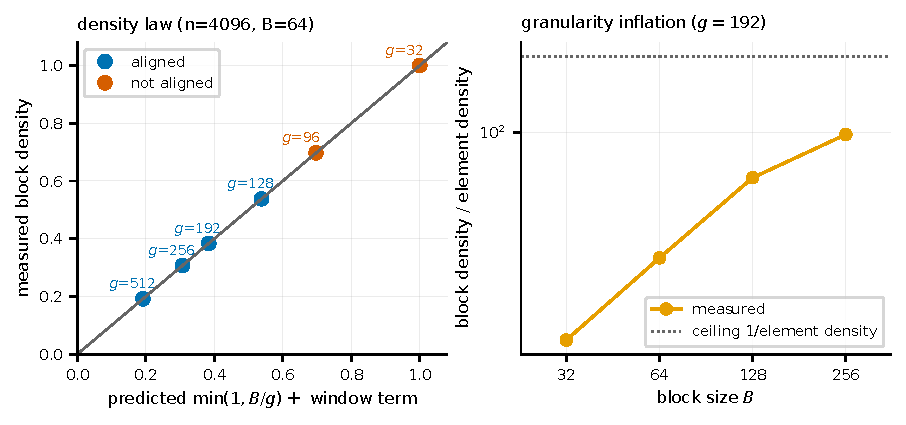
\includegraphics[width=\textwidth]{fig4_density.pdf}
\caption{Left: measured block density against the prediction
$\min(1,B/g)+$ window term; every point lies on the identity line, whether or not
the anchor period is a multiple of the block size. Right: ratio of block density
to element density against block size at fixed $g=192$; the dotted line is the
ceiling $1/$element density, reached when every block contains an anchor. Data:
\texttt{s1\_pswa/block\_alignment.json}.}
\label{fig:density}
\end{figure}

\subsection{The quality price, measured}\label{sec:mass}

Theorem~\ref{thm:mass} predicts an output deviation bounded by
$2(1-\rho)V_{\max}$. On the longest real entity sequence available in
\DatasetIeee{} we take $n=\QualityN$ ($w=\WinW$, $g=\AnchorG$, $s=\Sinks$) and
compute both sides. The mask retains $\rho=\RhoMean$ of the softmax mass on
average (minimum \RhoMin), so the deviation bound is \BoundMax{} with
$V_{\max}=\Vmax$; the measured maximum absolute output deviation is \EmpDiff, i.e.
\Tightness\% of the bound. The bound holds with slack and the slack is expected: it
is a worst-case statement over value vectors, whereas the measurement uses one
realised value matrix.

The number that matters for design is $\rho$ itself. A mask that keeps
\RhoMean{} of the mass discards $\EpsMean$ on average and up to \EpsMax{} for some
queries, and no kernel optimisation changes that: it is the geometric consequence
of a window of $\WinW$ positions on a sequence of $\QualityN$. Consistency between
this section and Section~\ref{sec:device} is not accidental: the same $w$ and $g$
are used, and the sparse implementation there is the implementation whose
deviation is bounded here.

\subsection{The data do not contain the period the mask assumes}\label{sec:acf}

The periodic anchor is only a modelling choice if some periodicity exists. We
therefore estimate the autocorrelation function of the real entity sequences
directly, on the \NSequences{} longest sequences, up to lag $200$. The spectrum is
dominated by short-range dependence: the lag-1 coefficient is \AcfLagOne, lag 2 is
roughly half of it, and the decay continues monotonically. There is a weak local
bump at lag \AcfWeakLag{} (\AcfWeakPeak), but it sits inside the tail of that decay
rather than above it. In the band around the period actually used,
$[\AnchorBandLo,\AnchorBandHi]$, the largest coefficient is at lag 65 and the
coefficient at $g=\AnchorG$ itself is \AcfAtG{} against a high-lag noise floor of
\AcfNoiseFloor{}: no periodic peak is significant.

The consequence is a scope condition, not a refutation of the mask. We use
$g=\AnchorG$ in every controlled experiment as a \emph{pre-registered control},
not as a learned parameter, and the artefact records
\texttt{g\_is\_data\_driven = false} beside those results. Anyone who reads the
device measurements as ``this period is right for this data'' would be
over-reading them; the measurements are about the cost of the pattern, and the
cost is the same for any period of the same size.

\subsection{Verdict, and what part of it is our implementation's fault}\label{sec:attn_disclose}

H1, H2, H3, H5 and H6 hold. H4 holds: on this device the anchor-based
implementation is worse than the fused dense kernel in both memory and latency at
every length where both run. We are careful about what H4 does and does not mean.

The measured cost of the anchor variant is the product of three factors: the
counting law (Prop.~\ref{prop:count}), the granularity inflation
(Prop.~\ref{prop:block}, measured at \BlockWorkInflation{}$\times$ the element
count at $B=\GpuBlock$ and $g=\GpuG$, i.e. between $B/2$ and $B$ while the window
term still contributes), and a padding factor of \PadFactor{} in our
batched kernel, which pads every query block to the
\MaxSelBlocks{} key blocks required by the last block instead of the
\MeanSelBlocks{} it needs on average. A hand-tuned kernel can remove the third
factor and part of the second, and we say so: the first two remain, and they are
properties of the family rather than of our code. Concretely, dividing the
measured memory and latency at $n=\LargestN$ by the padding factor leaves
\VramAfterDepad\,MiB and \LatAfterDepad\,ms, still far above the fused kernel's
\VramSdpaBig\,MiB and \LatSdpaBig\,ms. The ceiling of Corollary~\ref{cor:ceiling}
then bounds what any such kernel could achieve: a factor of $g/B=4$ at these
settings, against a mask that already keeps only \RhoMean{} of the mass.

We therefore scope the claim precisely. We do not claim that anchor-based sparsity
is asymptotically inferior to dense attention in arithmetic; we claim that (a) the
family is quadratic in the sequence length for any fixed period, (b) its arithmetic
advantage over dense attention is bounded by $g/B$, and (c) on a memory-constrained
device, with the implementation a practitioner would write from the published
description, it is dominated by a fused dense kernel at every length that device
can hold, while the same pattern without anchors is not. Claim (a) is proved,
claim (b) follows from the counting law and the granularity law, and claim (c) is
measured.

\subsection{A claim of ours that the apparatus refuted}\label{sec:attn_withdraw}

An earlier version of this work asserted a \emph{block-alignment lemma}: that
block-level sparsity requires the anchor period to be a multiple of the block
size, and that otherwise the pattern ``degenerates towards dense''. The claim was
false, and the way it failed is instructive enough to report.

The assertion that carried it compared the largest block density among unaligned
periods with twice the smallest among aligned ones. That is, it compared
\emph{different} values of $g$. On a steep grid the comparison is won by
construction, and the assertion held for reasons unrelated to the claim. The data
contradict it directly. At $B=\AlignBlock$ the aligned period $g=192$ gives a
block density of \WithdrawDensAligned{}, the unaligned period $g=96$ gives
\WithdrawDensUnaligned{}, and the densest row in the grid, $g=32$ at
\WithdrawDensDensest{}, is not a multiple of the block size at all. Density
tracks $g$, not alignment: a longer period is sparser whether or not it divides
the block size, and the densest row in the grid comes from $g<B$, which is a
different mechanism altogether. What survives is
\eqref{eq:blocklaw}: alignment does not change how many blocks are needed, it only
places the anchor on a block boundary, which matters for address arithmetic in a
streaming kernel and for nothing else.

We replaced the lemma with the counting law, re-ran the unit, and kept the flag
\url{former_lemma_withdrawn} in the result file so that a reader of the
artefact can see both versions. Section~\ref{sec:audit} explains why the apparatus
let a false claim through in the first place: the assertion and the hypothesis had
been merged, so the claim was encoded as something that had to be true.
